\documentclass[journal,12pt,onecolumn]{IEEEtran}
\usepackage{setspace}
\usepackage{gensymb}
\singlespacing
\usepackage[cmex10]{amsmath}
\usepackage{amsthm}
\usepackage{mathrsfs}
\usepackage{txfonts}
\usepackage{stfloats}
\usepackage{bm}
\usepackage{cite}
\usepackage{cases}
\usepackage{subfig}
\usepackage{longtable}
\usepackage{multirow}
\usepackage{enumitem}
\usepackage{mathtools}
\usepackage{tikz}
\usepackage{circuitikz}
\usepackage{verbatim}
\usepackage[breaklinks=true]{hyperref}
\usepackage{tkz-euclide} % loads  TikZ and tkz-base
\usepackage{listings}
\usepackage{color}    
\usepackage{array}    
\usepackage{longtable}
\usepackage{calc}     

\usepackage{hhline}   
\usepackage{ifthen}   
\usepackage{lscape}     
\usepackage{chngcntr}
\usepackage{float}
\DeclareMathOperator*{\Res}{Res}
\renewcommand\thesection{\arabic{section}}
\renewcommand\thesubsection{\thesection.\arabic{subsection}}
\renewcommand\thesubsubsection{\thesubsection.\arabic{subsubsection}}

\renewcommand\thesectiondis{\arabic{section}}
\renewcommand\thesubsectiondis{\thesectiondis.\arabic{subsection}}
\renewcommand\thesubsubsectiondis{\thesubsectiondis.\arabic{subsubsection}}
\renewcommand\thetable{\arabic{table}}
% correct bad hyphenation here
\hyphenation{op-tical net-works semi-conduc-tor}
\def\inputGnumericTable{}                                 %%

\lstset{
%language=C,
frame=single, 
breaklines=true,
columns=fullflexible
}
%\lstset{
%language=tex,
%frame=single, 
%breaklines=true
%}

\begin{document}
\newtheorem{theorem}{Theorem}[section]
\newtheorem{problem}{Problem}
\newtheorem{proposition}{Proposition}[section]
\newtheorem{lemma}{Lemma}[section]
\newtheorem{corollary}[theorem]{Corollary}
\newtheorem{example}{Example}[section]
\newtheorem{definition}[problem]{Definition}
\newcommand{\BEQA}{\begin{eqnarray}}
\newcommand{\EEQA}{\end{eqnarray}}
\newcommand{\define}{\stackrel{\triangle}{=}}
\bibliographystyle{IEEEtran}
\providecommand{\mbf}{\mathbf}
\providecommand{\pr}[1]{\ensuremath{\Pr\left(#1\right)}}
\providecommand{\qfunc}[1]{\ensuremath{Q\left(#1\right)}}
\providecommand{\sbrak}[1]{\ensuremath{{}\left[#1\right]}}
\providecommand{\lsbrak}[1]{\ensuremath{{}\left[#1\right.}}
\providecommand{\rsbrak}[1]{\ensuremath{{}\left.#1\right]}}
\providecommand{\brak}[1]{\ensuremath{\left(#1\right)}}
\providecommand{\lbrak}[1]{\ensuremath{\left(#1\right.}}
\providecommand{\rbrak}[1]{\ensuremath{\left.#1\right)}}
\providecommand{\cbrak}[1]{\ensuremath{\left\{#1\right\}}}
\providecommand{\lcbrak}[1]{\ensuremath{\left\{#1\right.}}
\providecommand{\rcbrak}[1]{\ensuremath{\left.#1\right\}}}
\theoremstyle{remark}
\newtheorem{rem}{Remark}
\newcommand{\sgn}{\mathop{\mathrm{sgn}}}
\providecommand{\abs}[1]{\left\vert#1\right\vert}
\providecommand{\res}[1]{\Res\displaylimits_{#1}} 
\providecommand{\norm}[1]{\left\lVert#1\right\rVert}
\providecommand{\mtx}[1]{\mathbf{#1}}
\providecommand{\mean}[1]{E\left[ #1 \right]}
\providecommand{\fourier}{\overset{\mathcal{F}}{ \rightleftharpoons}}
\providecommand{\system}[1]{\overset{\mathcal{#1}}{ \longleftrightarrow}}
\newcommand{\solution}{\noindent \textbf{Solution: }}
\newcommand{\cosec}{\,\text{cosec}\,}
\providecommand{\dec}[2]{\ensuremath{\overset{#1}{\underset{#2}{\gtrless}}}}
\newcommand{\myvec}[1]{\ensuremath{\begin{pmatrix}#1\end{pmatrix}}}
\newcommand{\mydet}[1]{\ensuremath{\begin{vmatrix}#1\end{vmatrix}}}
\let\vec\mathbf
\def\putbox#1#2#3{\makebox[0in][l]{\makebox[#1][l]{}\raisebox{\baselineskip}[0in][0in]{\raisebox{#2}[0in][0in]{#3}}}}
     \def\rightbox#1{\makebox[0in][r]{#1}}
     \def\centbox#1{\makebox[0in]{#1}}
     \def\topbox#1{\raisebox{-\baselineskip}[0in][0in]{#1}}
     \def\midbox#1{\raisebox{-0.5\baselineskip}[0in][0in]{#1}}

\vspace{3cm}
\title{}
\author{EE22BTECH11049 - Shivansh Kirar}
\maketitle
\textbf{Question EC 31 2023}\\
The signal-to-noise ratio (SNR) of an ADC with a full-scale sinusoidal input is given to be 61.96 dB. The resolution of the ADC is \hfill{GATE EC 2023}

\textbf{Solution:}
\begin{figure}[H]
  \centering
  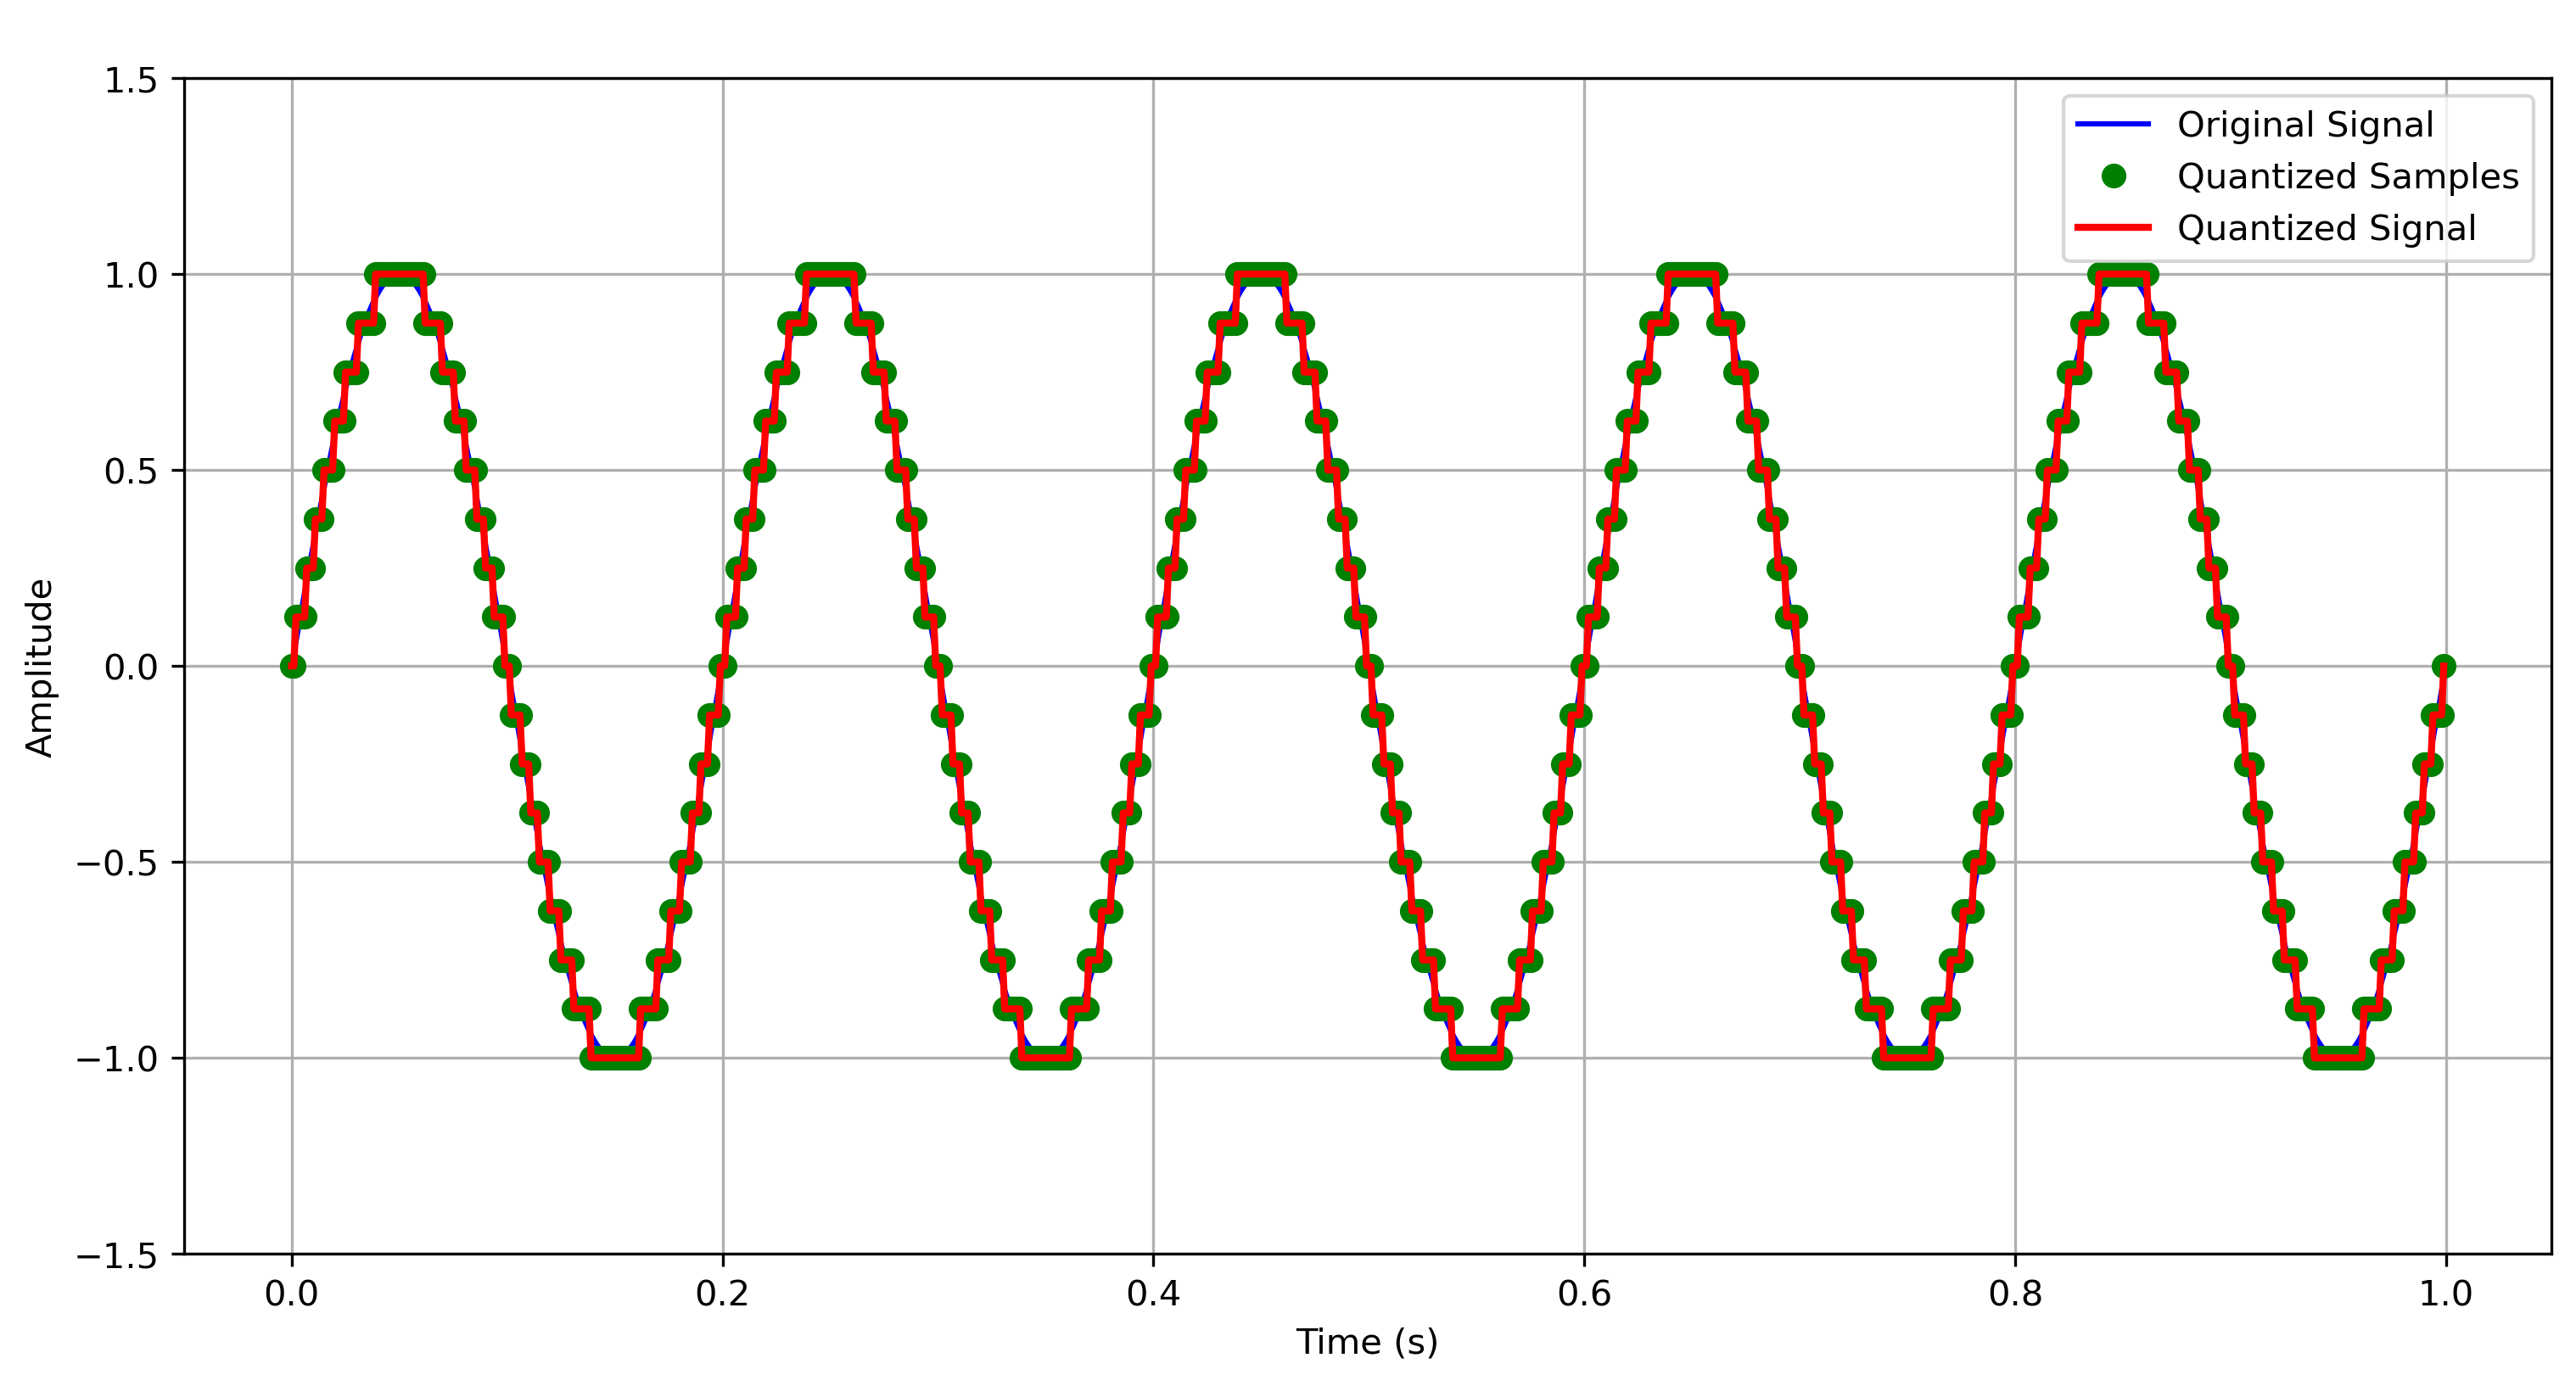
\includegraphics[width=1\textwidth]{Graph/a.png}
  \caption{Quantization of Sinusoidal Signal}
  \label{fig:Gate.31.2023}
\end{figure}
The mean power in a sinusoidal input signal with unit amplitude is simply
\begin{equation}
P_s = \frac{1}{T} \int_{0}^{T} \sin^2(\omega t) \, dt
\end{equation}
 where \(T\) is the time period of the signal, and \(\omega\) is the angular frequency.


Quantized to $2^n$ discrete levels, equivalent to $n$ bits, one quantization step $q$ has a size of
\begin{equation}
q = \frac{2}{2^{n}} = 2^{-(n-1)}
\end{equation}
We know,quantization error has a maximum value of plus or minus half the
step size, so 
\begin{equation}
\left| e \right| \leq \frac{q}{2} \text{ and therefore, } \left| e \right| \leq 2^{-n}
\end{equation}

For a large enough number of quantization steps, the probability density function of the quantization error tends toward being flat 1. Its value within the quantization error bounds is
\begin{equation}
p_e \approx \frac{1}{q}
\end{equation}

So, we can calculate its mean power or variance as the 2nd moment of its distribution.\\
Since, the distribution of error is uniform hence E[e]=0.
\begin{equation}
E[e^{2}] = \int_{-\frac{q}{2}}^{\frac{q}{2}} p(e) e^{2} \, de 
= \frac{1}{q} \cdot \frac{1}{3} \left(\left(\frac{q}{2}\right)^{3} - \left(-\frac{q}{2}\right)^{3}\right)
=\frac{1}{3q} \cdot \frac{q^{3}}{4}
=\frac{q^{2}}{12}
\end{equation}

On putting \(q = 2^{-(n-1)}\), we have:
\begin{equation}
E[e^{2}] \approx \frac{2^{-2n}}{3}
\end{equation}
\begin{equation}
P_e \approx \frac{2^{-2n}}{3}
\end{equation}
Thus, an ideal ADC would have a signal-to-noise ratio
\begin{equation}
SNR = \frac{P_s}{P_e} = 1.5 \cdot 2^{2n}
\end{equation}

or, expressed in decibels,
\begin{equation}
SNR = 1.76 + 6.02n
\end{equation}

Plug in the values:
\begin{equation}
n = \frac{61.96 \text{ dB} - 1.76 \text{ dB}}{6.02 \text{ dB}} \approx 10 \text{ bits}
\end{equation}

So, the resolution of the ADC is approximately 10 bits.
\end{document}
